\documentclass[11pt]{beamer}

% Minimalist theme settings
\usetheme{default}
\setbeamertemplate{navigation symbols}{}
\setbeamertemplate{footline}{}

% Smart Package Loading
\usepackage{amsmath}
\usepackage{amssymb}
\usepackage{tikz}
\usetikzlibrary{shapes.geometric, arrows.meta, positioning, calc, decorations.pathreplacing}

\begin{document}
	
	\begin{frame}{Equation 1}
		\begin{equation}
			\mathbf{s}_t = \begin{bmatrix} a_{t-1} \\ r_{t-1} \end{bmatrix} \in \mathbb{R}^{2}
		\end{equation}
		
		\vfill
		\begin{center}
			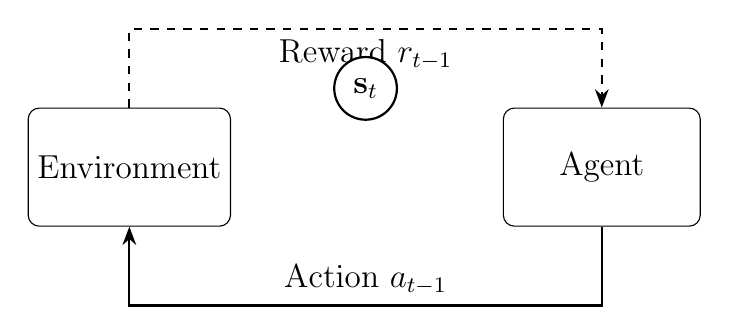
\begin{tikzpicture}[>=Stealth, font=\large]
				\node[draw, rectangle, rounded corners, minimum height=1.5cm, minimum width=2.5cm, fill=white] (env) at (0,0) {Environment};
				\node[draw, rectangle, rounded corners, minimum height=1.5cm, minimum width=2.5cm, fill=white] (agent) at (6,0) {Agent};
				
				\draw[->, thick] (agent.south) -- ++(0,-1) -| (env.south) node[near start, above] {Action $a_{t-1}$};
				\draw[->, thick, dashed] (env.north) -- ++(0,1) -| (agent.north) node[near start, below] {Reward $r_{t-1}$};
				
				\node[draw, circle, fill=white, thick, inner sep=4pt] at (3, 1) {$\mathbf{s}_t$};
			\end{tikzpicture}
		\end{center}
	\end{frame}
	
	\begin{frame}{Equation 2}
		\begin{equation}
			u_{t, j} = 
			\begin{cases} 
				\sigma(\beta_j \cdot s_{t, c_j}) & d_j = 0 \text{ (Tonic)} \\
				\sigma(\beta_j \cdot (s_{t, c_j} - s_{t-d_j, c_j})) & d_j > 0 \text{ (Phasic)}
			\end{cases}
		\end{equation}
		
		\vfill
		\begin{center}
			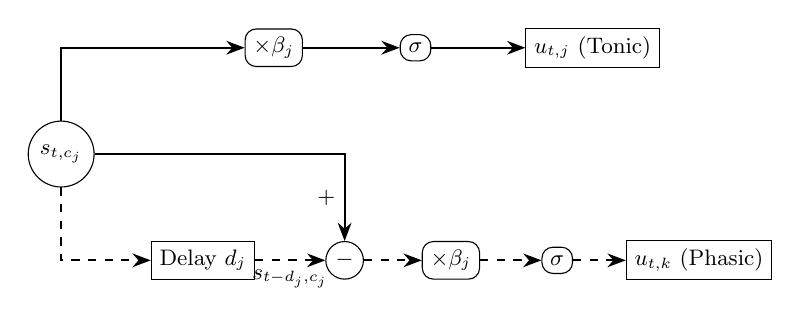
\begin{tikzpicture}[>=Stealth, font=\small, scale=0.9, transform shape]
				\node[draw, circle, inner sep=3pt, fill=white] (s) at (0, 0) {$s_{t, c_j}$};
				
				% Tonic path
				\node[draw, rectangle, rounded corners, fill=white] (beta1) at (3, 1.5) {$\times \beta_j$};
				\node[draw, rectangle, rounded corners, fill=white] (sig1) at (5, 1.5) {$\sigma$};
				\node[draw, rectangle, fill=white] (u1) at (7.5, 1.5) {$u_{t, j}$ (Tonic)};
				
				\draw[->, thick, solid] (s) |- (beta1);
				\draw[->, thick, solid] (beta1) -- (sig1);
				\draw[->, thick, solid] (sig1) -- (u1);
				
				% Phasic path
				\node[draw, rectangle, fill=white] (delay) at (2, -1.5) {Delay $d_j$};
				\node[draw, circle, inner sep=2pt, fill=white] (sub) at (4, -1.5) {$-$};
				\node[draw, rectangle, rounded corners, fill=white] (beta2) at (5.5, -1.5) {$\times \beta_j$};
				\node[draw, rectangle, rounded corners, fill=white] (sig2) at (7, -1.5) {$\sigma$};
				\node[draw, rectangle, fill=white] (u2) at (9, -1.5) {$u_{t, k}$ (Phasic)};
				
				\draw[->, thick, dashed] (s) |- (delay);
				\draw[->, thick, dashed] (delay) -- (sub) node[midway, below] {$s_{t-d_j, c_j}$};
				\draw[->, thick, solid] (s) -| (sub) node[near end, left] {$+$};
				\draw[->, thick, dashed] (sub) -- (beta2);
				\draw[->, thick, dashed] (beta2) -- (sig2);
				\draw[->, thick, dashed] (sig2) -- (u2);
			\end{tikzpicture}
		\end{center}
	\end{frame}
	
	\begin{frame}{Equation 3}
		\begin{equation}
			\mathbf{W}_{in} \in \mathbb{R}^{N_{GC} \times d_{channels}} \quad \text{(CSR, Row-Degree} = 4)
		\end{equation}
		
		\vfill
		\begin{center}
			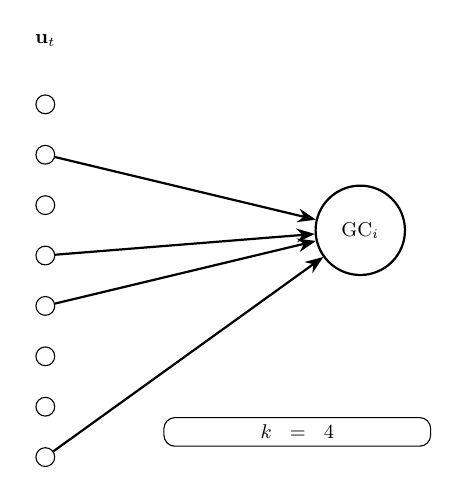
\begin{tikzpicture}[>=Stealth, font=\small, scale=0.8, transform shape]
				% Mossy Fiber Array
				\node[above] at (0, 4.5) {$\mathbf{u}_t$};
				\foreach \i in {1,2,3,4,5,6,7,8} {
					\node[draw, circle, inner sep=3pt, fill=white] (mf\i) at (0, 4.5 - \i*0.8) {};
				}
				
				% Granule Cell
				\node[draw, circle, inner sep=8pt, fill=white, thick] (gc) at (5, 1.7) {GC$_i$};
				
				% 4 Claws
				\draw[->, thick, solid] (mf2) -- (gc);
				\draw[->, thick, solid] (mf4) -- (gc);
				\draw[->, thick, solid] (mf5) -- (gc);
				\draw[->, thick, solid] (mf8) -- (gc);
				
				% Labels
				\node[draw, rectangle, rounded corners, align=center, fill=white, text width=4cm] at (4, -1.5) {$k=4$};
			\end{tikzpicture}
		\end{center}
	\end{frame}
	
	\begin{frame}{Equation 4}
		\begin{equation}
			\Delta t_t = X_{\text{ITI}, t-1} + X_{\text{RT}, t}
		\end{equation}
		
		\vfill
		\begin{center}
			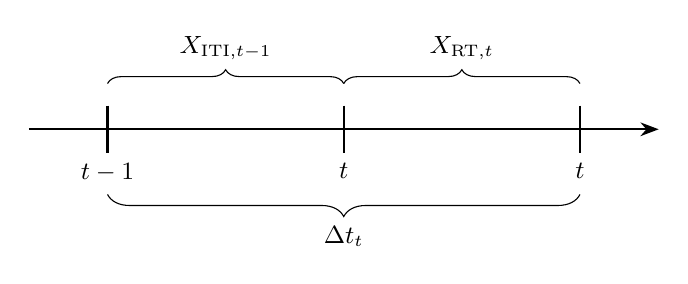
\begin{tikzpicture}[>=Stealth, font=\small]
				\draw[->, thick] (0,0) -- (8,0);
				
				\draw[thick] (1, 0.3) -- (1, -0.3) node[below] {$t-1$};
				\draw[thick] (4, 0.3) -- (4, -0.3) node[below] {$t$};
				\draw[thick] (7, 0.3) -- (7, -0.3) node[below] {$t$};
				
				\draw[decorate, decoration={brace, amplitude=5pt}, yshift=8pt] (1,0.3) -- (4,0.3) node[midway, above, yshift=5pt] {$X_{\text{ITI}, t-1}$};
				
				\draw[decorate, decoration={brace, amplitude=5pt}, yshift=8pt] (4,0.3) -- (7,0.3) node[midway, above, yshift=5pt] {$X_{\text{RT}, t}$};
				
				\draw[decorate, decoration={brace, amplitude=8pt, mirror}, yshift=-15pt] (1,-0.3) -- (7,-0.3) node[midway, below, yshift=-8pt] {$\Delta t_t$};
			\end{tikzpicture}
		\end{center}
	\end{frame}
	
	\begin{frame}{Equation 5}
		\begin{equation}
			\boldsymbol{\Gamma}(\Delta t_t) = \boldsymbol{\rho}_{base} + (\mathbf{1} - \boldsymbol{\rho}_{base}) \odot \exp \left( -\frac{\Delta t_t}{\boldsymbol{\tau}} \right)
		\end{equation}
		
		\vfill
		\begin{center}
			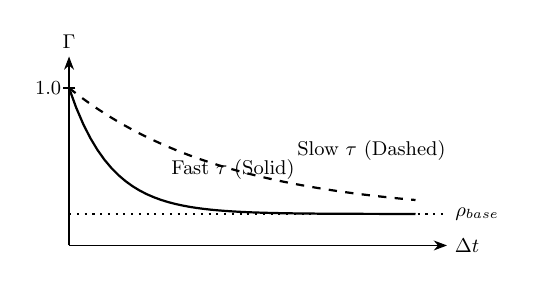
\begin{tikzpicture}[>=Stealth, font=\small, scale=0.8, transform shape]
				\draw[->] (0,0) -- (6,0) node[right] {$\Delta t$};
				\draw[->] (0,0) -- (0,3) node[above] {$\Gamma$};
				\draw[dotted, thick] (0, 0.5) -- (6, 0.5) node[right] {$\rho_{base}$};
				\node[left] at (0, 2.5) {$1.0$};
				\draw (0.1, 2.5) -- (-0.1, 2.5);
				
				\draw[thick, solid, domain=0:5.5, samples=50] plot (\x, {0.5 + 2*exp(-1.5*\x)});
				\draw[thick, dashed, domain=0:5.5, samples=50] plot (\x, {0.5 + 2*exp(-0.4*\x)});
				
				\node[right] at (1.5, 1.2) {Fast $\tau$ (Solid)};
				\node[right] at (3.5, 1.5) {Slow $\tau$ (Dashed)};
			\end{tikzpicture}
		\end{center}
	\end{frame}
	
	\begin{frame}{Equation 6}
		\begin{equation}
			\mathbf{h}_{pre, t} = \tanh \left( \mathbf{W}_{in} \mathbf{u}_t + \boldsymbol{\Gamma}(\Delta t_t) \odot \mathbf{z}_{GC, t-1} \right)
		\end{equation}
		
		\vfill
		\begin{center}
			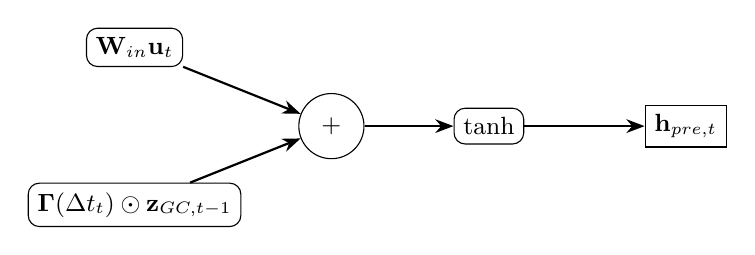
\begin{tikzpicture}[>=Stealth, font=\small]
				\node[draw, rectangle, rounded corners, fill=white] (w_u) at (0, 1) {$\mathbf{W}_{in} \mathbf{u}_t$};
				\node[draw, rectangle, rounded corners, fill=white] (decay) at (0, -1) {$\boldsymbol{\Gamma}(\Delta t_t) \odot \mathbf{z}_{GC, t-1}$};
				\node[draw, circle, inner sep=5pt, fill=white] (sum) at (2.5, 0) {$+$};
				\node[draw, rectangle, rounded corners, fill=white] (tanh) at (4.5, 0) {$\tanh$};
				\node[draw, rectangle, fill=white] (out) at (7, 0) {$\mathbf{h}_{pre, t}$};
				
				\draw[->, thick] (w_u) -- (sum);
				\draw[->, thick] (decay) -- (sum);
				\draw[->, thick] (sum) -- (tanh);
				\draw[->, thick] (tanh) -- (out);
			\end{tikzpicture}
		\end{center}
	\end{frame}
	
	\begin{frame}{Equation 7}
		\begin{equation}
			\mathbf{z}_{GoC, t} = \text{ReLU} \left( \mathbf{W}_{fb} \mathbf{h}_{pre, t} + \mathbf{W}_{collateral} \mathbf{y}_{t-1} \right)
		\end{equation}
		
		\vfill
		\begin{center}
			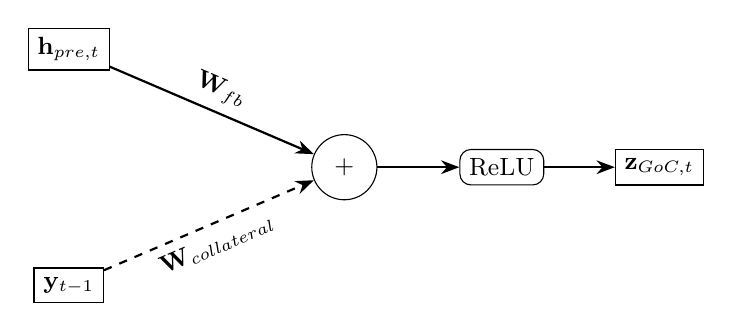
\begin{tikzpicture}[>=Stealth, font=\small]
				\node[draw, rectangle, fill=white] (hpre) at (0, 1.5) {$\mathbf{h}_{pre, t}$};
				\node[draw, rectangle, fill=white] (y) at (0, -1.5) {$\mathbf{y}_{t-1}$};
				
				\node[draw, circle, inner sep=5pt, fill=white] (sum) at (3.5, 0) {$+$};
				\node[draw, rectangle, rounded corners, fill=white] (relu) at (5.5, 0) {ReLU};
				\node[draw, rectangle, fill=white] (zgoc) at (7.5, 0) {$\mathbf{z}_{GoC, t}$};
				
				\draw[->, thick, solid] (hpre) -- (sum) node[midway, above, sloped] {$\mathbf{W}_{fb}$};
				\draw[->, thick, dashed] (y) -- (sum) node[midway, below, sloped] {$\mathbf{W}_{collateral}$};
				\draw[->, thick] (sum) -- (relu);
				\draw[->, thick] (relu) -- (zgoc);
			\end{tikzpicture}
		\end{center}
	\end{frame}
	
	\begin{frame}{Equation 8}
		\begin{equation}
			\mathbf{z}_{GC, t} = \max(0, \mathbf{h}_{pre, t} - \mathbf{W}_{inh} \mathbf{z}_{GoC, t})
		\end{equation}
		
		\vfill
		\begin{center}
			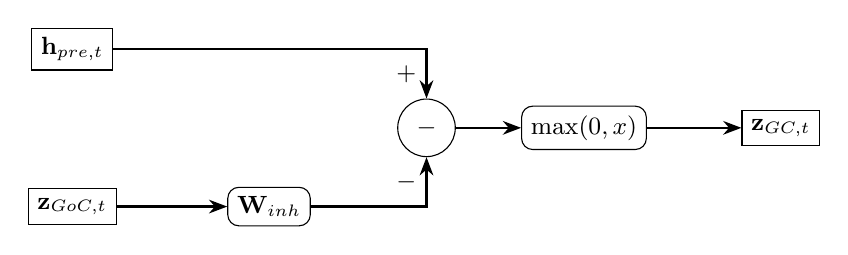
\begin{tikzpicture}[>=Stealth, font=\small]
				\node[draw, rectangle, fill=white] (hpre) at (0, 1) {$\mathbf{h}_{pre,t}$};
				\node[draw, rectangle, fill=white] (zgoc) at (0, -1) {$\mathbf{z}_{GoC,t}$};
				
				\node[draw, rectangle, rounded corners, fill=white] (winh) at (2.5, -1) {$\mathbf{W}_{inh}$};
				\node[draw, circle, inner sep=4pt, fill=white] (sub) at (4.5, 0) {$-$};
				
				\node[draw, rectangle, rounded corners, fill=white] (max) at (6.5, 0) {$\max(0, x)$};
				\node[draw, rectangle, fill=white] (out) at (9, 0) {$\mathbf{z}_{GC, t}$};
				
				\draw[->, thick] (hpre) -| (sub) node[near end, left] {$+$};
				\draw[->, thick] (zgoc) -- (winh);
				\draw[->, thick] (winh) -| (sub) node[near end, left] {$-$};
				\draw[->, thick] (sub) -- (max);
				\draw[->, thick] (max) -- (out);
			\end{tikzpicture}
		\end{center}
	\end{frame}
	
	\begin{frame}{Equation 9}
		\begin{equation}
			V_t = \sigma \left( \mathbf{w}_v^\top \mathbf{z}_{GC, t} \right)
		\end{equation}
		
		\vfill
		\begin{center}
			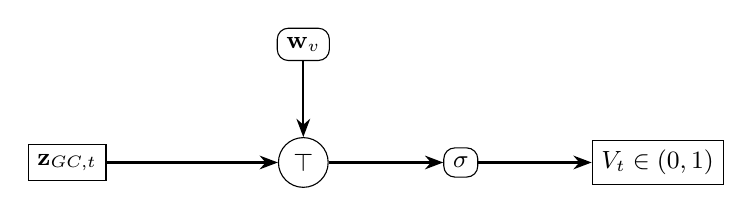
\begin{tikzpicture}[>=Stealth, font=\small]
				\node[draw, rectangle, fill=white] (z) at (0, 0) {$\mathbf{z}_{GC, t}$};
				\node[draw, circle, inner sep=3pt, fill=white] (dot) at (3, 0) {$\top$};
				\node[draw, rectangle, rounded corners, fill=white] (wv) at (3, 1.5) {$\mathbf{w}_v$};
				\node[draw, rectangle, rounded corners, fill=white] (sig) at (5, 0) {$\sigma$};
				\node[draw, rectangle, fill=white] (v) at (7.5, 0) {$V_t \in (0,1)$};
				
				\draw[->, thick] (z) -- (dot);
				\draw[->, thick] (wv) -- (dot);
				\draw[->, thick] (dot) -- (sig);
				\draw[->, thick] (sig) -- (v);
			\end{tikzpicture}
		\end{center}
	\end{frame}
	
	\begin{frame}{Equation 10}
		\begin{equation}
			\boldsymbol{\pi}_t = \text{Softmax}(\mathbf{W}_\pi \mathbf{z}_{GC, t})
		\end{equation}
		
		\vfill
		\begin{center}
			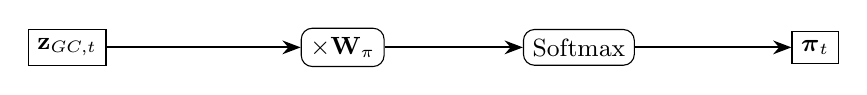
\begin{tikzpicture}[>=Stealth, font=\small]
				\node[draw, rectangle, fill=white] (z) at (0, 0) {$\mathbf{z}_{GC, t}$};
				\node[draw, rectangle, rounded corners, fill=white] (wp) at (3.5, 0) {$\times \mathbf{W}_\pi$};
				\node[draw, rectangle, rounded corners, fill=white] (sm) at (6.5, 0) {Softmax};
				\node[draw, rectangle, fill=white] (pi) at (9.5, 0) {$\boldsymbol{\pi}_t$};
				
				\draw[->, thick] (z) -- (wp);
				\draw[->, thick] (wp) -- (sm);
				\draw[->, thick] (sm) -- (pi);
			\end{tikzpicture}
		\end{center}
	\end{frame}
	
	\begin{frame}{Equation 11}
		\begin{equation}
			\mathbf{e}_{t} = \boldsymbol{\Gamma}(\Delta t_t) \odot \mathbf{z}_{GC, t}
		\end{equation}
		
		\vfill
		\begin{center}
			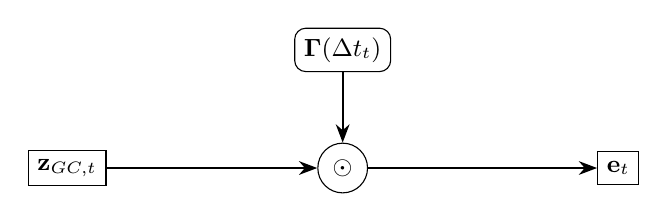
\begin{tikzpicture}[>=Stealth, font=\small]
				\node[draw, rectangle, fill=white] (z) at (0, 0) {$\mathbf{z}_{GC, t}$};
				\node[draw, circle, inner sep=3pt, fill=white] (had) at (3.5, 0) {$\odot$};
				\node[draw, rectangle, rounded corners, fill=white] (gamma) at (3.5, 1.5) {$\boldsymbol{\Gamma}(\Delta t_t)$};
				\node[draw, rectangle, fill=white] (e) at (7, 0) {$\mathbf{e}_t$};
				
				\draw[->, thick] (z) -- (had);
				\draw[->, thick] (gamma) -- (had);
				\draw[->, thick] (had) -- (e);
			\end{tikzpicture}
		\end{center}
	\end{frame}
	
	\begin{frame}{Equation 12}
		\begin{equation}
			S_t = -\sum p_{t,i} \log(p_{t,i}) \quad \Rightarrow \quad \Omega_t = \exp \left( -k_{entropy} \cdot S_t \right)
		\end{equation}
		
		\vfill
		\begin{center}
			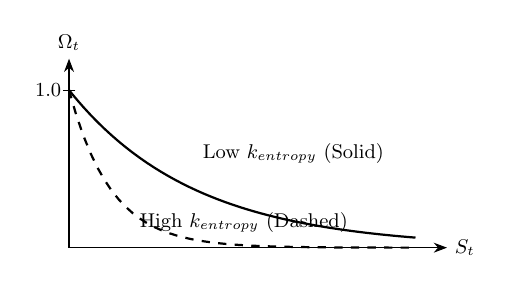
\begin{tikzpicture}[>=Stealth, font=\small, scale=0.8, transform shape]
				\draw[->] (0,0) -- (6,0) node[right] {$S_t$};
				\draw[->] (0,0) -- (0,3) node[above] {$\Omega_t$};
				
				\draw[thick, solid, domain=0:5.5, samples=50] plot (\x, {2.5*exp(-0.5*\x)});
				\draw[thick, dashed, domain=0:5.5, samples=50] plot (\x, {2.5*exp(-1.5*\x)});
				
				\node[right] at (2, 1.5) {Low $k_{entropy}$ (Solid)};
				\node[right] at (1, 0.4) {High $k_{entropy}$ (Dashed)};
				\node[left] at (0, 2.5) {$1.0$};
				\draw (0.1, 2.5) -- (-0.1, 2.5);
			\end{tikzpicture}
		\end{center}
	\end{frame}
	
	\begin{frame}{Equation 13}
		\begin{equation}
			\mathbf{w}_{v, t+1} = \max \left( 0, \mathbf{w}_{v, t} + \eta \cdot \Omega_t \cdot \delta_t \cdot \mathbf{e}_{t} \right)
		\end{equation}
		
		\vfill
		\begin{center}
			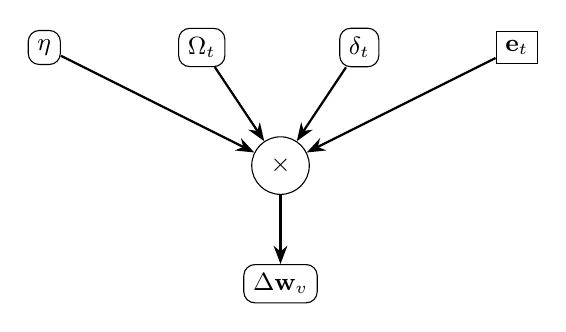
\begin{tikzpicture}[>=Stealth, font=\small]
				\node[draw, rectangle, rounded corners, fill=white] (eta) at (0, 1.5) {$\eta$};
				\node[draw, rectangle, rounded corners, fill=white] (omega) at (2, 1.5) {$\Omega_t$};
				\node[draw, rectangle, rounded corners, fill=white] (delta) at (4, 1.5) {$\delta_t$};
				\node[draw, rectangle, fill=white] (e) at (6, 1.5) {$\mathbf{e}_t$};
				
				\node[draw, circle, inner sep=4pt, fill=white] (prod) at (3, 0) {$\times$};
				
				\node[draw, rectangle, rounded corners, fill=white] (w) at (3, -1.5) {$\Delta \mathbf{w}_v$};
				
				\draw[->, thick] (eta) -- (prod);
				\draw[->, thick] (omega) -- (prod);
				\draw[->, thick] (delta) -- (prod);
				\draw[->, thick] (e) -- (prod);
				
				\draw[->, thick] (prod) -- (w);
			\end{tikzpicture}
		\end{center}
	\end{frame}
	
\end{document}